% =====================================================================================
%  Chapter 3 — Method
%  Self-contained. Nothing to \input. Requires thesis/references.bib.
%
%  PREAMBLE (already in main.tex): graphicx, booktabs, multirow, threeparttable, amsmath
%  ASSETS: figures/fig_spheres.pdf, figures/fig_shield_block.pdf
%    Regenerate both:  PYTHONPATH=. python -m experiments.make_fig_method
%
%  THIS CHAPTER DEFINES THE TWO LABELS CHAPTER 4 HAS BEEN REFERENCING AND FAILING TO RESOLVE:
%    \label{sec:metrics}  (Section 3.1, Metrics)
%    \label{sec:barrier}  (Section 3.2, Obstacle geometry and the barrier)
%  It also defines sec:shield, referenced from Chapter 2.
%
%  FIVE PROPERTIES OF THE BARRIER ARE STATED IN 3.2 RATHER THAN DISCOVERED IN CHAPTER 4.
%  Do not trim them for length: 4.5's fidelity argument, 4.2's comparison against the
%  published baseline, and 5.3's limitations all cite them. Removing them makes those
%  sections read as post-hoc excuses rather than anticipated consequences.
% =====================================================================================

\chapter{Method}\label{ch:method}

\section{The SafeLIBERO Benchmark}\label{sec:benchmark}

All experiments use SafeLIBERO~\cite{vlsa2026}, which augments the LIBERO manipulation
suite~\cite{liu2023libero} with non-target obstacles placed in the workspace. The grid is three
task suites (spatial, object, goal) $\times$ two obstacle levels $\times$ four tasks, giving 24
distinct scenes, each providing 50 randomised initial states.

Initial states 0--34 are used for demonstration collection and training; states 35--49 are held out
and used only for evaluation. Every result in Chapter~\ref{ch:results} evaluates five held-out
initial states per scene, giving $n = 120$ rollouts per condition. Rollouts run for a horizon of
300 control steps, with the policy queried every five steps and the next five actions of the
emitted chunk executed before the next query.

\subsection{Metrics}\label{sec:metrics}

\paragraph{Task success rate (TSR)} is the fraction of rollouts in which the environment's own goal
predicate, compiled from each task's BDDL specification, is satisfied at any point before the
horizon expires. That predicate is treated as authoritative throughout; a geometric fallback
present in the codebase for logging is disabled for every number reported. Success is binary per
rollout.

\paragraph{Collision} is recorded when the obstacle's position departs from its position at the
start of the episode by more than one millimetre in the $\ell_1$ sense,
\begin{equation}
  \sum_{k \in \{x,y,z\}} \bigl| p_k(t) - p_k(0) \bigr| > 0.001~\mathrm{m},
  \label{eq:collision}
\end{equation}
and a rollout is marked collided if this holds at any control step. Three properties of the
definition matter. It is \emph{cumulative} against the episode's initial pose rather than a
per-step contact test, so an obstacle nudged early stays flagged. It measures the obstacle being
\emph{displaced} rather than being touched by the robot, so an obstacle knocked over by the carried
payload counts --- the quantity of interest is disturbance of the scene. And the reference pose
$p(0)$ is taken after the settling procedure of Section~\ref{sec:benchmark_fixes}, since objects
otherwise cross the threshold under gravity before the policy has acted.
\textbf{Collision-avoidance rate (CAR)} is the complement.

The one-millimetre $\ell_1$ threshold is this work's operationalisation. The originating work
defines its collision metric as the proportion of strictly collision-free episodes and states no
numeric tolerance~\cite{vlsa2026}, so the threshold here was chosen to sit above simulator noise
while remaining strict enough that no genuine contact passes it. It is not inherited from that
work.

\paragraph{Execution time to success (ETS)} is the control step at which the success predicate
first holds, averaged over successful rollouts only and reported in control steps. Failed rollouts
are excluded rather than assigned the horizon: substituting the horizon would make a policy appear
\emph{faster} the more often it fails. ETS is therefore conditional on success and must be read
alongside TSR. The originating work uses the same name for a different quantity --- mean episode
length including timeouts --- so values here are internally comparable but not comparable to
theirs.

\paragraph{CBF activation rate} is the fraction of control steps on which the shield altered the
action, counted whenever the projected action differs from the nominal by more than $10^{-4}$ in
norm. It measures how \emph{often} the shield intervened, not how large the corrections were, and
serves as an independent check on internalisation: a policy that has learned to avoid obstacles
should need fewer corrections when the shield is reattached.

All proportions are reported with 95\% Wilson score confidence intervals rather than normal
approximations. At $n = 120$ with rates near zero or one --- where several of these results sit ---
the normal approximation gives intervals that are too narrow and can extend outside $[0,1]$.

\section{Obstacle Geometry and the Barrier}\label{sec:barrier}

The obstacle's collision mesh is read from the simulator, sampled into a point cloud, and decomposed
into a small set of spheres. Sphere decomposition is used rather than a single bounding volume
because a bounding sphere over a non-convex object is a poor approximation: an earlier version of
this work measured a 5.5\,cm carton as 16\,cm across, enough to distort the grasp it produced
(Figure~\ref{fig:spheres}a).

\begin{figure}[htbp]
  \centering
  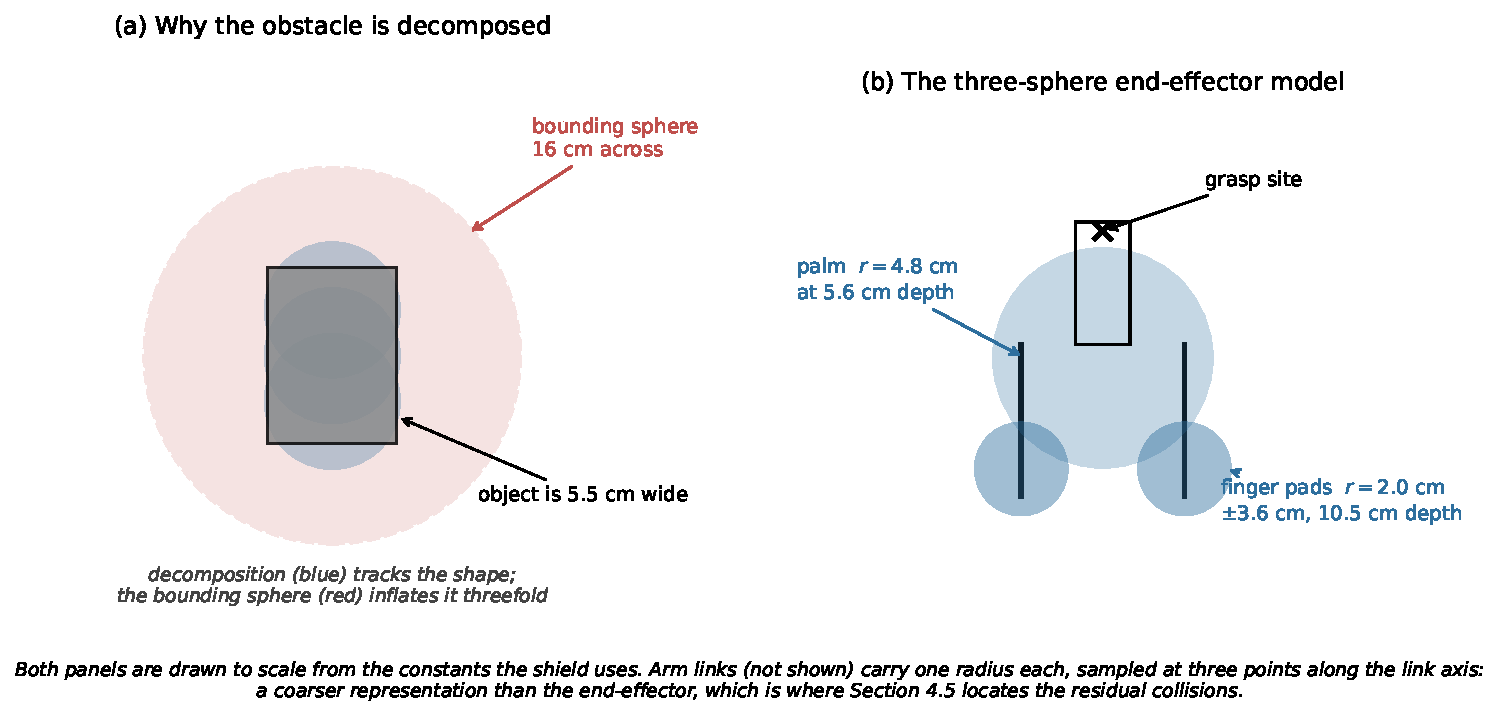
\includegraphics[width=\linewidth]{figures/fig_spheres.pdf}
  \caption[The geometric model used by the barrier]{%
    The geometric model, drawn to scale from the constants the shield uses.
    \textbf{(a)} A single bounding sphere inflates a 5.5\,cm object to 16\,cm; decomposition tracks
    the shape.
    \textbf{(b)} The three-sphere end-effector model. Arm links, not shown, carry one radius each
    sampled at three points along the link axis --- a coarser representation, which
    Section~\ref{sec:res:scope} identifies as where residual collisions concentrate.}
  \label{fig:spheres}
\end{figure}

The robot is represented by spheres on both sides of the barrier.

\paragraph{End-effector.} Three spheres in the end-effector frame approximate the Franka hand: a
palm sphere of radius 4.8\,cm at 5.6\,cm behind the grasp site, and two finger-pad spheres of
radius 2.0\,cm offset 3.6\,cm either side at 10.5\,cm depth. A single sphere would either miss the
fingers or inflate the palm.

\paragraph{Arm links.} Links three through seven and the hand body are each assigned a radius
(5.5\,cm to 9.0\,cm, set from the link's maximum transverse extent plus a 15--21\,mm margin) and
sampled at three positions along the link axis, so a long link is not represented by its origin
alone.

For each pair of a robot sphere $i$ and an obstacle sphere $j$ the barrier is
\begin{equation}
  h_{ij} = \lVert p_i - c_j \rVert^{2} - (r_i + r_j)^{2},
  \label{eq:barrier}
\end{equation}
with $h > 0$ the safe set. Differentiating along the rigid-body velocity gives the constraint row
\begin{equation}
  \bigl[\, 2\,s\,(p_i - c_j)^{\top} R_1 \,\bigr]\, u \;+\; k\,h_{ij} \;\ge\; 0,
  \qquad k = 10,
  \label{eq:constraint_row}
\end{equation}
where $u$ is the commanded end-effector velocity in the body frame, $R_1$ its rotation and $s$ a
scale factor. For arm links, whose velocity is not the commanded one, the mapping
$v_{\mathrm{link}} \approx J_{\mathrm{link}} J_{\mathrm{ee}}^{+}\,(s R_1 u)$ is used, with
$J_{\mathrm{ee}}^{+}$ a damped pseudo-inverse ($\lambda = 10^{-3}$).

Five properties of this construction bear on Chapter~\ref{ch:results} and are stated here rather
than discovered later.

\begin{itemize}
  \item \emph{The robot model is approximate, and unevenly so.} The end-effector is covered by
  three fitted spheres; each arm link by three point samples carrying one radius. The end-effector
  is represented considerably more faithfully than the links.

  \item \emph{Links one and two are not constrained at all}, being close to the base and rarely
  near the obstacle in these scenes.

  \item \emph{Arm-link velocities are estimated, not commanded.} The quadratic program optimises an
  end-effector velocity and infers each link's motion through a damped Jacobian pseudo-inverse.
  Where that inverse is ill-conditioned --- near singularities, or when the null-space motion the
  operational-space controller applies differs from the minimum-norm solution --- the predicted
  link velocity and the realised one diverge, and the constraint is enforced against the
  prediction.

  \item \emph{The geometry is privileged.} Obstacle poses and sizes are read from the simulator
  rather than estimated from the policy's observations. The originating work instead derives
  obstacle geometry through vision-language grounding and fused depth, and attributes its residual
  collisions primarily to that upstream pipeline rather than to the controller~\cite{vlsa2026}. The
  figures reported here are therefore an upper bound for this class of filter.

  \item \emph{Arm links are constrained here but not in the originating work}, whose formulation
  solely constrains the end-effector and which notes that its unconstrained kinematic links may
  consequently collide~\cite{vlsa2026}. Extending the barrier to the links is a deliberate
  difference from that baseline, and Section~\ref{sec:shield_efficacy} reports its effect.
\end{itemize}

\section{The CBF Shield}\label{sec:shield}

At each control step the policy's proposed translation is treated as a nominal end-effector
velocity $u_{\mathrm{nom}}$, and the shield solves
\begin{equation}
  u^{\star} = \arg\min_{u} \lVert u - u_{\mathrm{nom}} \rVert^{2}
  \quad \text{s.t.} \quad
  a_m^{\top} u + b_m \ge 0 \;\; \text{for every constraint row } m,
  \label{eq:shield_qp}
\end{equation}
a quadratic program in three variables whose rows are the end-effector/obstacle and arm-link pairs
of Section~\ref{sec:barrier}. This is the standard CBF-QP form~\cite{ames2017cbf}, instantiated on
the sphere-pair barrier of Equation~\ref{eq:barrier}; that sphere construction is this work's own
simplification rather than an adoption of an existing distance formulation. When no constraint is
active the solution is $u_{\mathrm{nom}}$ and the action passes through unchanged.

\begin{figure}[htbp]
  \centering
  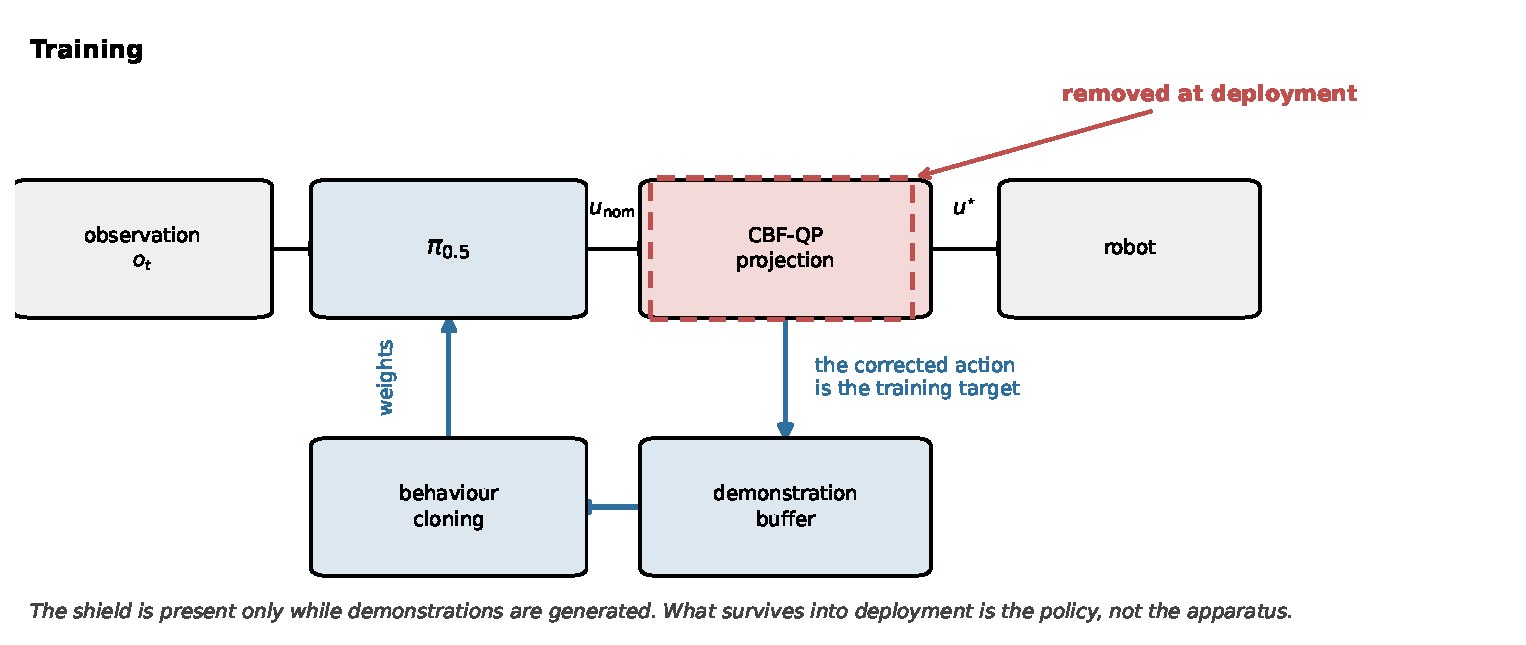
\includegraphics[width=\linewidth]{figures/fig_shield_block.pdf}
  \caption[The shield, and what it leaves behind]{%
    The shield during demonstration collection. The policy proposes, the quadratic program
    projects, the robot executes --- and the corrected action is tapped off as the imitation
    target. The distinction this work draws is what happens next: the projection block is deleted
    at deployment, and what remains is the policy alone.}
  \label{fig:shield_block}
\end{figure}

The problem is solved with OSQP~\cite{stellato2020osqp} through
CVXPY~\cite{diamond2016cvxpy}; where CVXPY is unavailable the implementation falls back to SLSQP
and, if that fails, to the unconstrained action while emitting a warning --- a silent fallback
would be indistinguishable from a shield that was never needed. An intervention is recorded when
the returned action differs from the nominal by more than $10^{-4}$, which is what the CBF
activation rate of Section~\ref{sec:metrics} counts.

Two discrete-time adjustments are required because the barrier's guarantee is continuous-time. The
effective radius is inflated by a lag buffer covering the distance travelled between control steps
and the inverse-kinematics tracking error; this value was tuned upward during development after
collisions were observed at nominally safe margins. Rotation is not constrained: the barrier acts
on the translational channel only.

\section{Collision Attribution}\label{sec:attribution}

The headline collision metric answers \emph{whether} the obstacle moved, not \emph{what} moved it.
Because the barrier's authority is uneven across the robot, the distinction is essential to
interpreting the residual, so each episode additionally records which bodies contacted the
obstacle, grouped as gripper, arm link, held object, and other scene objects.

Two cautions apply and are observed throughout Chapter~\ref{ch:results}. Contacts with other scene
objects fire on essentially every episode, including collision-free ones, because an obstacle
resting on its supporting surface registers a permanent contact; that category is excluded from
analysis rather than interpreted. And the contact-graph attribution is a documented lower bound ---
it can miss delayed or indirect pushes --- so demonstration filtering uses the raw displacement
flag rather than the attributed one, which is the stricter choice.

\section{Teachers}\label{sec:teachers}

Two sources of demonstrations are compared, and the comparison between them is the central
experiment of this work.

\subsection{The Shielded Policy as Its Own Teacher}\label{sec:teacher_self}

The policy is rolled out with the shield active, and episodes are retained if they succeeded,
displaced nothing, and the shield intervened at least once. That third criterion matters: a clean
episode in which the shield never fired is ordinary base-policy behaviour and teaches nothing about
safety. Because the corrections are applied to actions the policy itself proposed, the
demonstrations are located at states the policy actually reaches --- the property
Section~\ref{sec:res:source} identifies as decisive.

\subsection{A Privileged Scripted Expert}\label{sec:teacher_planner}

The alternative teacher is a sampling-based motion planner: RRT-Connect in joint space with
clearance inflation, followed by inverse kinematics and playback as operational-space deltas. It
reads object and goal poses directly from the BDDL scene specification~\cite{liu2023libero}, and is
safe by construction rather than by correction. Unlike the shielded policy, it plans from its own
initial conditions and is never conditioned on where $\pi_{0.5}$ fails.

\subsection{Why \texorpdfstring{$\pi_{0.5}$}{pi 0.5}, and What Was Tried First}
\label{sec:base_choice}

The base policy was not the first choice, and the reason for changing it bears on how the results
should be read. The work began on OpenVLA-7B with a Cartesian CBF filter, and the first
distillation attempt collected CBF-corrected demonstrations and fine-tuned that model through LoRA.
It produced no useful learning signal.

Two causes were identified, and only one is about the model. The shield was mis-configured at the
time of collection, so the corrected actions differed only marginally from the base policy's own
proposals --- the dataset nominally contained corrections but carried almost no correction signal,
a failure mode invisible to any check that counts demonstrations rather than measuring how much
they were changed. Separately, OpenVLA-7B's base competence on LIBERO is low enough that safety and
capability failures are difficult to separate: a policy that rarely completes the task provides
little opportunity to observe whether it completes it \emph{safely}.

Both considerations pointed to the same change. $\pi_{0.5}$ has substantially stronger base LIBERO
performance, which makes the safety question well-posed, and it is the policy the runtime-shielding
baseline evaluates~\cite{vlsa2026}, which makes the comparison in
Section~\ref{sec:shield_efficacy} direct. The episode is recorded because it is the origin of a
check used throughout: demonstration sets are audited for how much the shield actually changed
them, not merely for whether they were collected successfully.

\section{Distillation}\label{sec:distillation}

Retained demonstrations are behaviour-cloned using the model's native flow-matching
loss~\cite{physicalintelligence2025pi05,black2024pi0}. Only the parameters selected by the training
configuration's trainable filter receive gradients --- a LoRA adapter on the action head --- while
the vision-language backbone is frozen; the saved artefact is the adapter alone, reapplied over the
base checkpoint at load time. The imitation target is the sequence of actions actually executed,
that is post-shield, so the policy learns the corrected behaviour rather than its own original
proposals. Actions are normalised by passing them through the policy's own input transform, so the
target matches the distribution the model was pretrained on rather than a hand-rolled
normalisation.

The procedure sits in the DAgger lineage~\cite{ross2011dagger}, and shares with
SafeDAgger~\cite{zhang2017safedagger} the idea that a safe controller's interventions are
themselves the informative signal. It is not a new algorithm; the contribution of this work is
empirical, and Chapter~\ref{ch:background} says so explicitly.

\paragraph{Comparing training runs.}
Where two distilled policies are compared they are matched on \textbf{gradient steps}, not epochs.
This is necessary because episode length differs between teachers: a shielded rollout at horizon
300 yields roughly 35 training examples, while a planner episode at horizon 900 yields roughly 412.
Matching epochs would have given one policy 16{,}140 gradient steps and the other approximately
212{,}000, which is not a controlled comparison but a different experiment. The two students
compared in Section~\ref{sec:res:source} were trained for 16{,}140 and 15{,}988 steps respectively.

\section{Two Corrections to the Benchmark}\label{sec:benchmark_fixes}

Two defects in the simulation had to be fixed before any measurement was trustworthy; both are
reported with their evidence in Section~\ref{sec:res:benchmark}. Unused obstacles are parked
off-scene by SafeLIBERO in a heap dense enough to overflow MuJoCo's contact buffer, and on overflow
contacts are discarded order-dependently, making episodes non-reproducible. Separately, objects
spawned in unsupported poses fall under gravity while the arm is stationary, and that displacement
is charged to the robot.

The fixes are to clear collision flags on parked bodies and to allow the scene to settle before
measurement begins --- in that order, since settling before the first fix reintroduces the
non-determinism it is meant to precede.
